\section{Implementação}

\subsection{Detalhes da implementação}

Para a implementação do trabalho com objetivo de criar um método para resolver o problema de determinar o número máximo de caminhos disjuntos em arestas existentes em um grafo, utilizamos três principais pontos, dentre eles os três que serão explicados e deslindados abaixo.


% Matriz de adjacência
\subsubsection{Matriz de Adjacência}
Para inserir os grafos no algoritmo utilizamos matrizes de adjacências, utilizando sempre o peso 1 para as arestas, tendo como objetivo que cada aresta só pode ter um uso durante o encontro do caminho disjunto.

Exemplo de Matriz de Adjacência para o seguinte Grafo:

\begin{center}
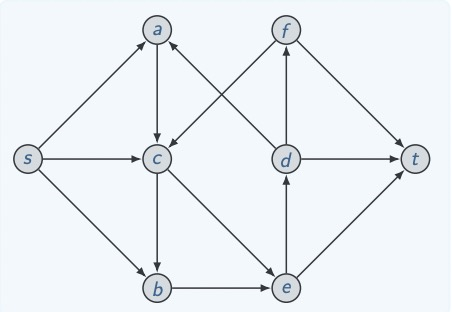
\includegraphics[height=4cm]{figuras/04.jpg}
\end{center}

\begin{scriptsize}
\estiloR
\begin{lstlisting}[title={Matriz de Adjacência para o Grafo acima}, label=lst:javacode]
grafo = [
#    0, 1, 2, 3, 4, 5, 6, 7
    [0, 1, 1, 1, 0, 0, 0, 0], # 0
    [0, 0, 1, 0, 0, 0, 0, 0], # 1
    [0, 0, 0, 1, 0, 0, 1, 0], # 2
    [0, 0, 0, 0, 0, 0, 1, 0], # 3
    [0, 0, 1, 0, 0, 0, 0, 1], # 4
    [0, 1, 0, 0, 1, 0, 0, 1], # 5
    [0, 0, 0, 0, 0, 1, 0, 1], # 6
    [0, 0, 0, 0, 0, 0, 0, 0]  # 7
]
\end{lstlisting}
\end{scriptsize}


\subsubsection{Ford-Fulkerson}

Com a finalidade de utilizar um algoritmo que tenha, nesse caso, um resultado ótimo, optei por utilizar o algoritmo de Ford-Fulkerson, seguindo pelos princípios e normas já citado acima ele se caracteriza como uma base adequada para a resolução do problema apresentado.

\begin{scriptsize}
\estiloJava
\begin{lstlisting}[title={Algoritmo baseado no Ford-Fulkerson}, label=lst:javacode, language=Python]
# Aplicacao do algoritimo do ford fulkerson adaptado para o problema
# metodo de resolucao deste problema que receba um grafo e um par de vértices
def caminhos_disjuntos(self, origem, destino):
    parent = [-1] * (self.ROW)
    max_caminhos_disjuntos = 0
    
    while self.busca_bfs(origem, destino, parent):
        original_destino = destino;
        caminho = [];
        path = float("Inf")
        s = destino
        
        while(s != origem):
            path = min(path, self.graph[parent[s]][s])
            s = parent[s]
            caminho.append(s);
        
        # Adicionar o fluxo ao grafo
        max_caminhos_disjuntos += 1   
        # atualizar o grafo residual com o fluxo
        v = destino
        while(v != origem):
            u = parent[v]
            self.graph[u][v] -= path
            self.graph[v][u] += path
            v = parent[v]
        res_caminho = caminho[::-1]           #Formatacao do caminho para printar corretamente
        res_caminho.append(original_destino)
        string_caminho = [str(int) for int in res_caminho]

        print(' -> '.join(string_caminho)) # print do caminho

    print("Maximo de caminhos disjuntos encontrados: %d " % max_caminhos_disjuntos)

    return max_caminhos_disjuntos
\end{lstlisting}
\end{scriptsize}


\subsubsection{Busca em Largura}

Pensando de que, diferentemente do Best Finding Search e outros algoritmos que podem deletar arestas e/ou causar uma "confusão" nos caminhos já passados, optei por implementar uma busca em largura, na qual armazena as arestas -  já vistadas a partir de um determinado vértice $s$, tendo por direção um vértice $t$, - e uma lista incrementada até que o vértice definido por $t$ seja alcançado.

\begin{scriptsize}
\estiloJava
\begin{lstlisting}[title={Algoritmo BFS}, label=lst:javacode, language=Python]
# Utilizar uma BFS como um algoritmo de busca
def busca_bfs(self, s, t, parent):
    ja_visitado = [False] * (self.ROW)
    lista = []

    lista.append(s)
    ja_visitado[s] = True

    while lista:
        u = lista.pop(0)
        for ind, val in enumerate(self.graph[u]):
            if ja_visitado[ind] == False and val > 0:
                lista.append(ind)
                ja_visitado[ind] = True
                parent[ind] = u


    return True if ja_visitado[t] else False
\end{lstlisting}
\end{scriptsize}

\subsection{Replit.com}
Para executar o código do algoritmo e os testes implementados, você poderá rodar em sua maquina utilizando os arquivos que estão com código fonte, utilizando do seguinte comando: \textbf{python index.py} ou rodar pelo Replit, uma plataforma para compartilhar códigos fontes e a execução, para que possamos minimizar o problema de incompatibilidade do programa com alguma arquitetura, ou configurações de compiladores diferentes. 
\\
https://replit.com/@GustavoBretas/Trabalho2Grafos